\section{Arquitetura do sistema}
\subsection{Modelo OAIS}
O nosso sistema será construido seguindo as orientações do modelo OAIS \textit{(Open Archival Information System)} da Figura ~\ref{fig:oais}

\begin{figure}[H] 
  \centering
  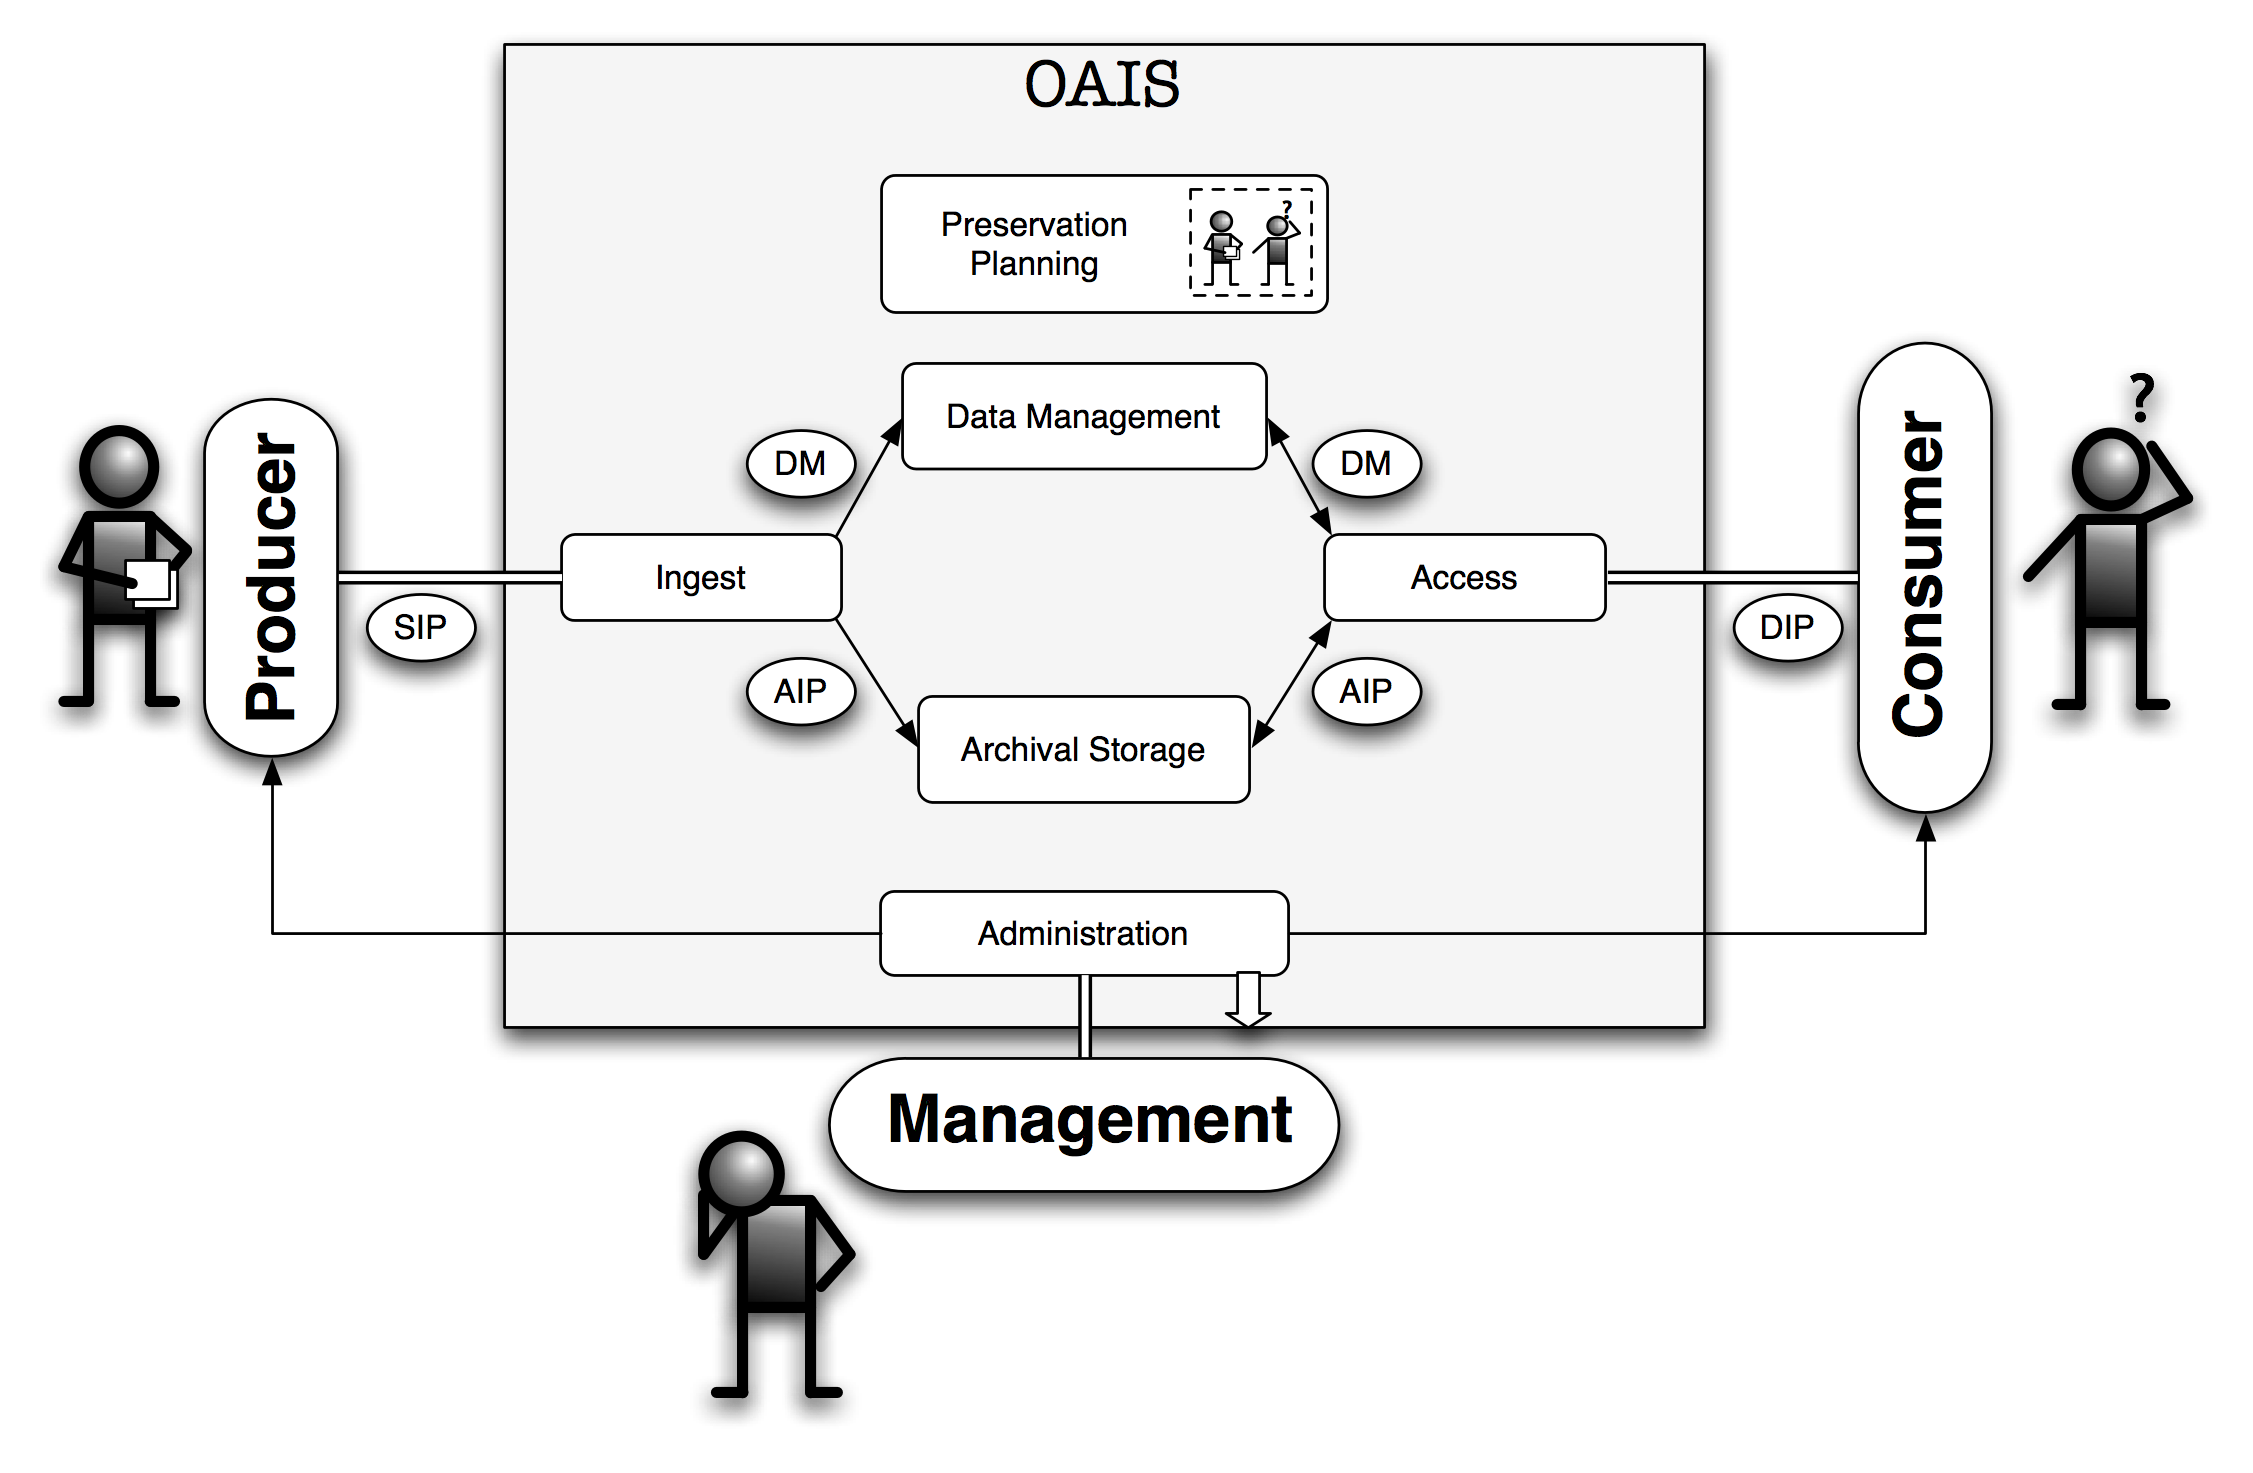
\includegraphics[width=1\textwidth,center]{images/arquitetura/oais}
  \caption{Modelo OAIS}
  \label{fig:oais}
\end{figure}

Como representado na Figura ~\ref{fig:oais}, o sistema irá interagir com três tipos distintos de atores:
\begin{description}[labelindent=1cm]
  \item[Produtores] que serão representados pelos Alunos.
  \item[Administrador] que serão representados pelos Docentes.
  \item[Consumidor] que serão representados pelos Utilizadores não Registados.
\end{description}
E será constituido por três mega processos:
\begin{description}[labelindent=1cm]
  \item[Ingestão] responsável pela receção e depósito de projetos.
  \item[Administração] responsável pela gestão interna do sistema.
  \item[Disseminação] responsável pela disseminação, distribuição e publicação dos objetos arquivados.
\end{description}

\subsection{Fluxo do Sistema}

Com o objetivo de perceber e organizar melhor o fluxo do nosso sistema, construimos um \textbf{Diagrama de Atividade} que de uma forma pouco pormenorizada demonstra sequencialmente as principais ações dos utilizadores do sistema. De notar que este diagrama será importante para perceber a ligação entre os vários utilizadores e as ações dependentes entre estes.

Com o \textbf{Diagrama de Atividade} da Figura ~\ref{fig:diagrama-blocos}, podemos consultar de forma simplificada o fluxo do nosso sistema.

\begin{figure}[H] 
  \centering
  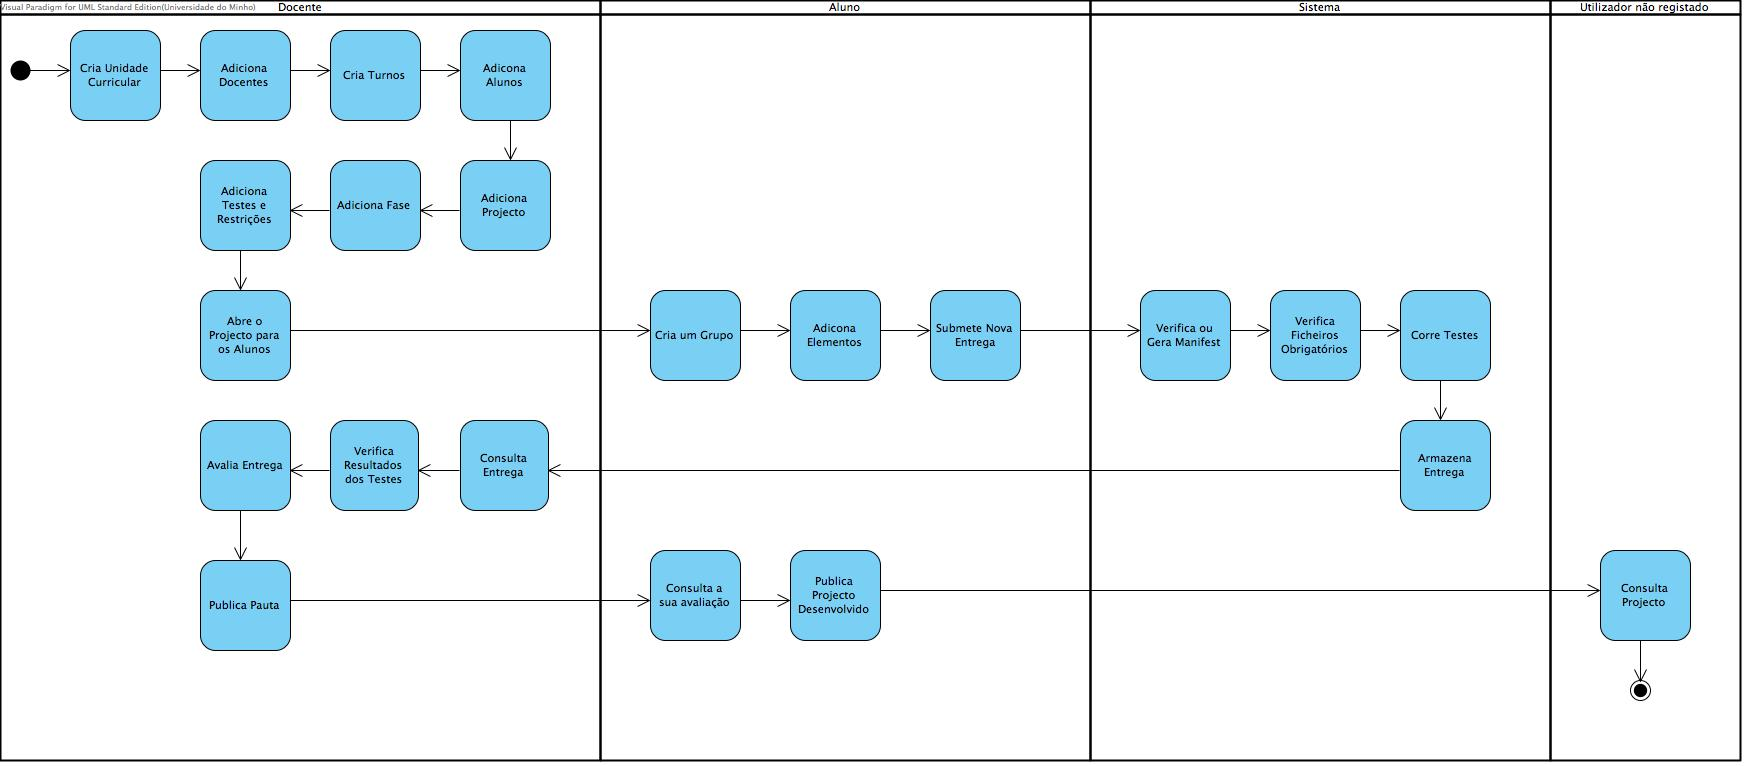
\includegraphics[width=1\textwidth,center]{images/arquitetura/diagrama-blocos}
  \caption{Fluxo do Sistema}
  \label{fig:diagrama-blocos}
\end{figure}

Para a representação do fluxo das funcionalidades mais complexas da aplicação, construiu-se \textbf{Diagramas de Atividade} que permitem representar essas mesmas funcionalidades mais pormenorizadamente.
Estes diagramas para além de ajudarem a perceber melhor o funcionamento do sistema nas tarefas mais relevantes, serão um excelente apoio na implementação do sistema.

Na Figura ~\ref{fig:criacao-projecto} podemos consultar o fluxo de criação de um projeto, desde o acesso ao sistema por parte de um docente, até ao acesso à página do projeto por parte de um aluno.

\begin{figure}[H] 
  \centering
  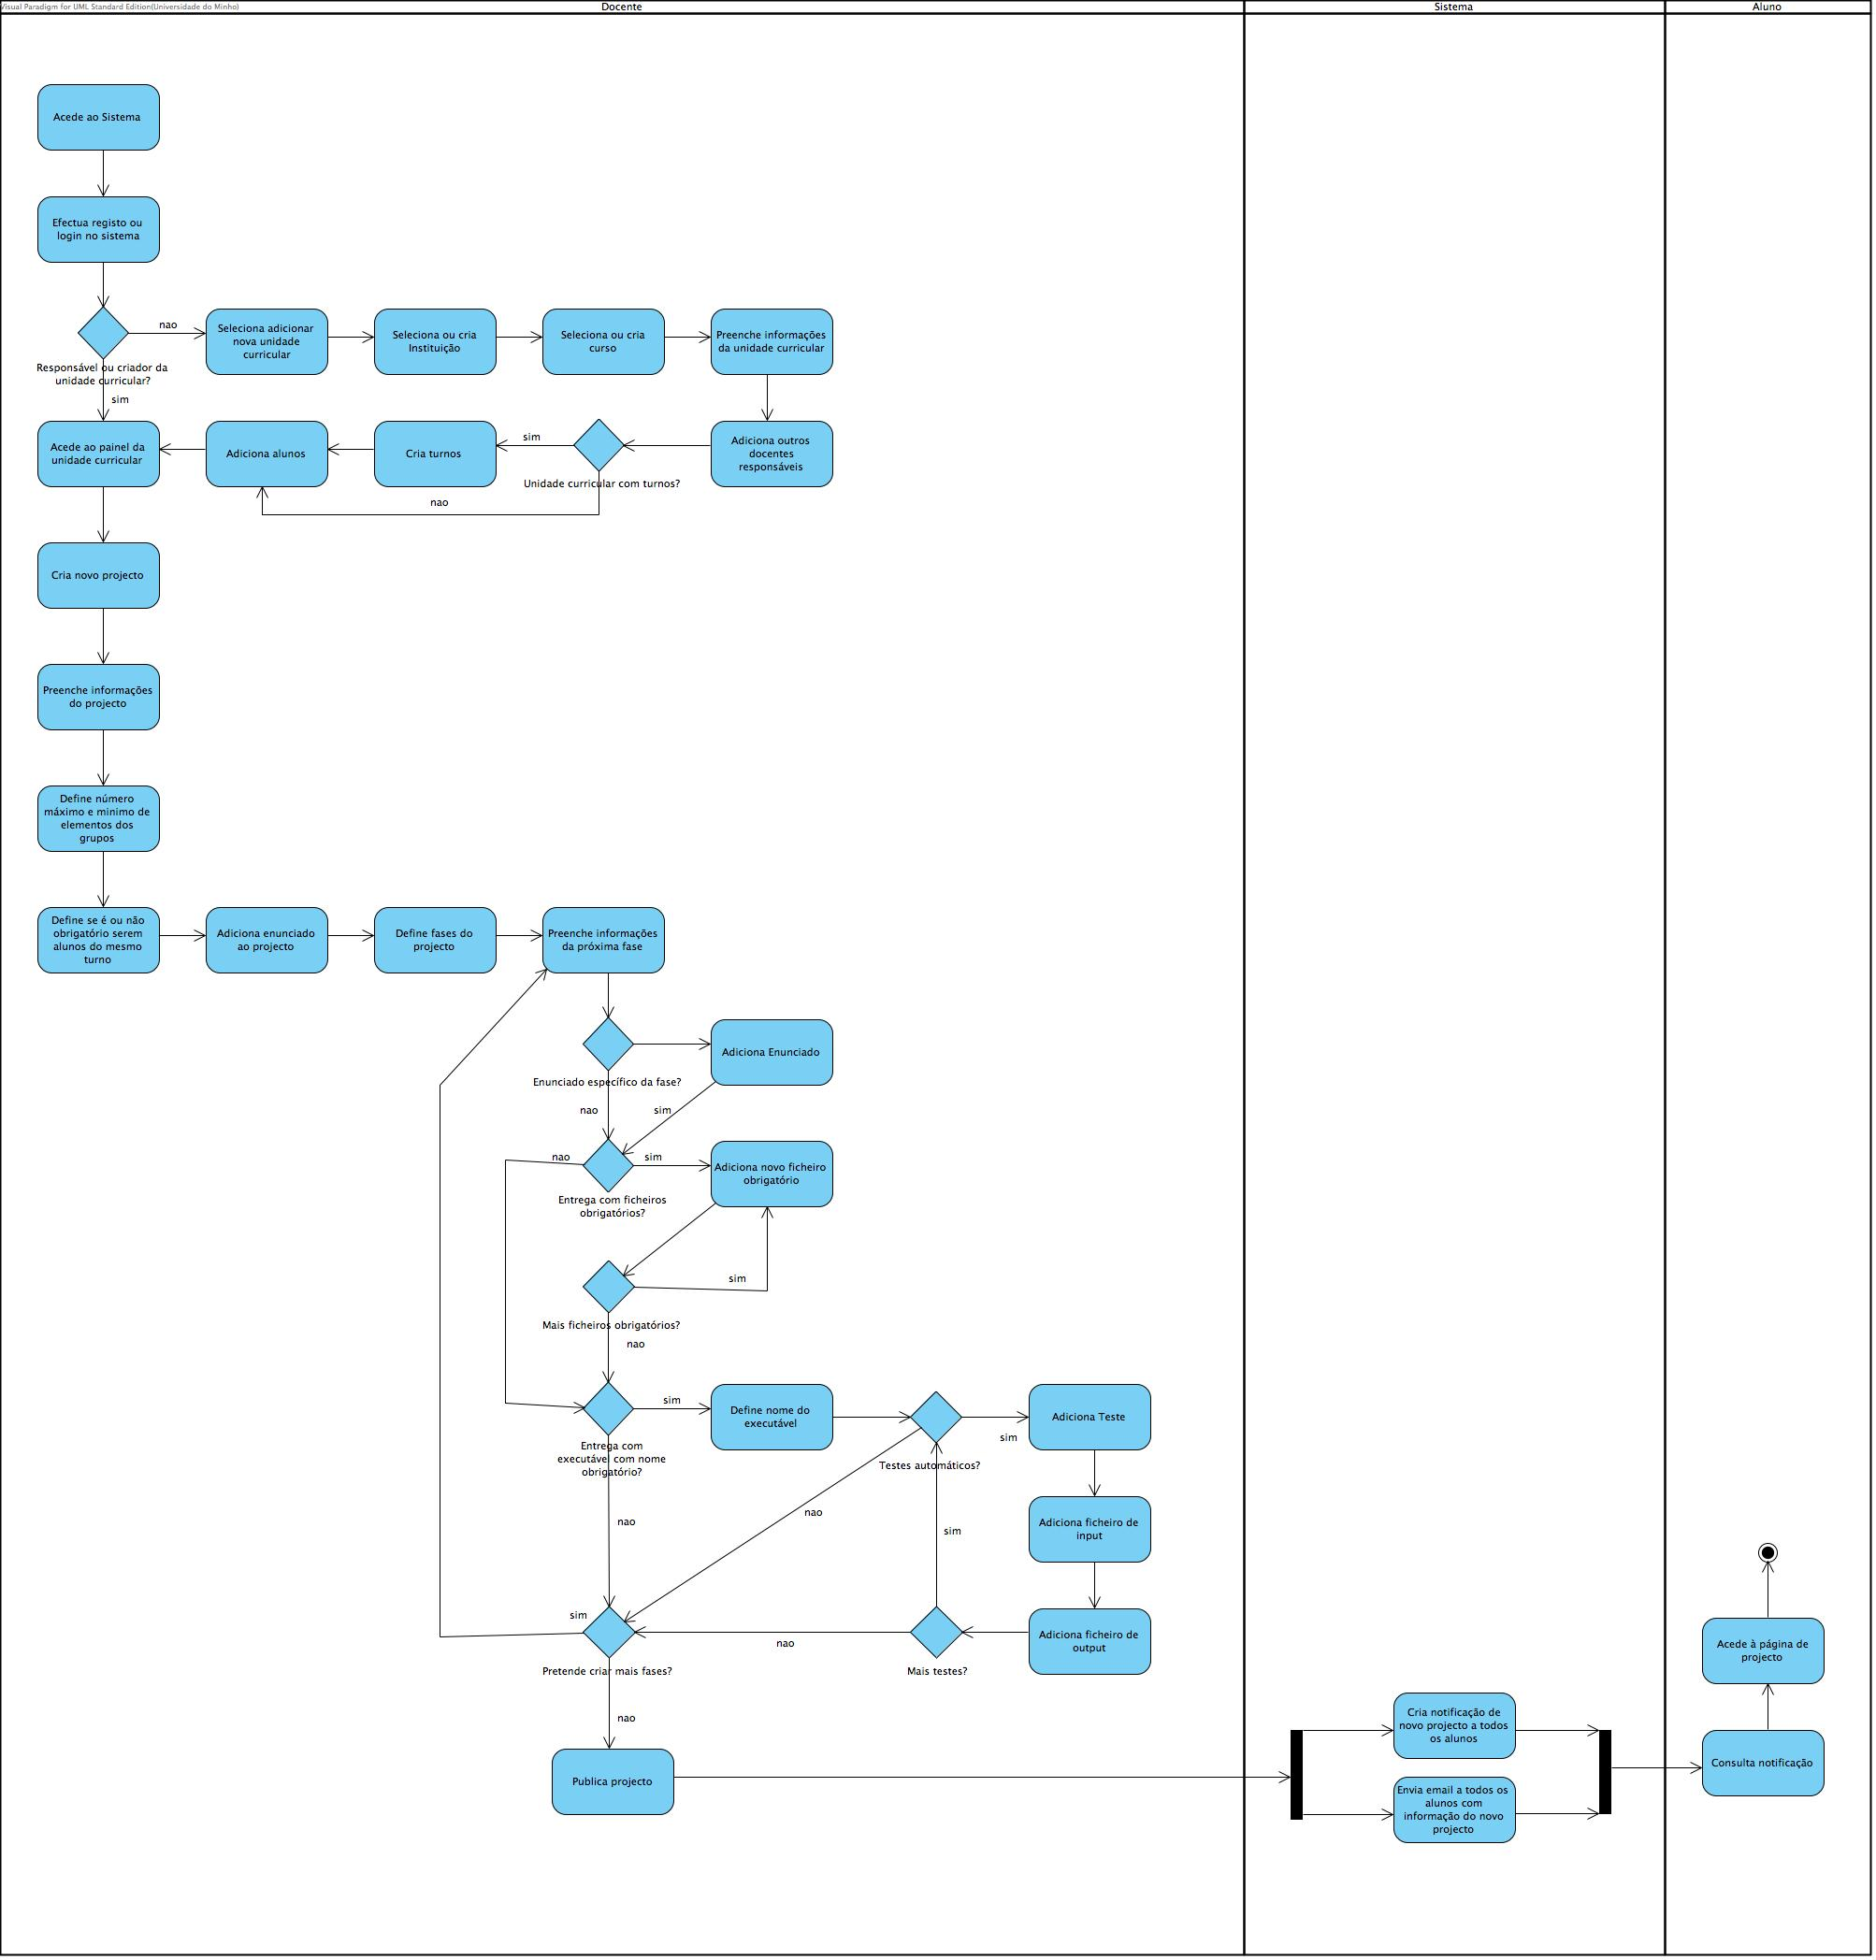
\includegraphics[width=1\textwidth,center]{images/arquitetura/criacao-projecto}
  \caption{Fluxo: Criar Projecto}
  \label{fig:criacao-projecto}
\end{figure}

Na Figura ~\ref{fig:submissao-projecto} podemos consultar o fluxo de submissão de um projeto, desde o acesso à página de um projeto por parte de um utilizador até à consulta das informações da entrega por parte de um docente.

\begin{figure}[H] 
  \centering
  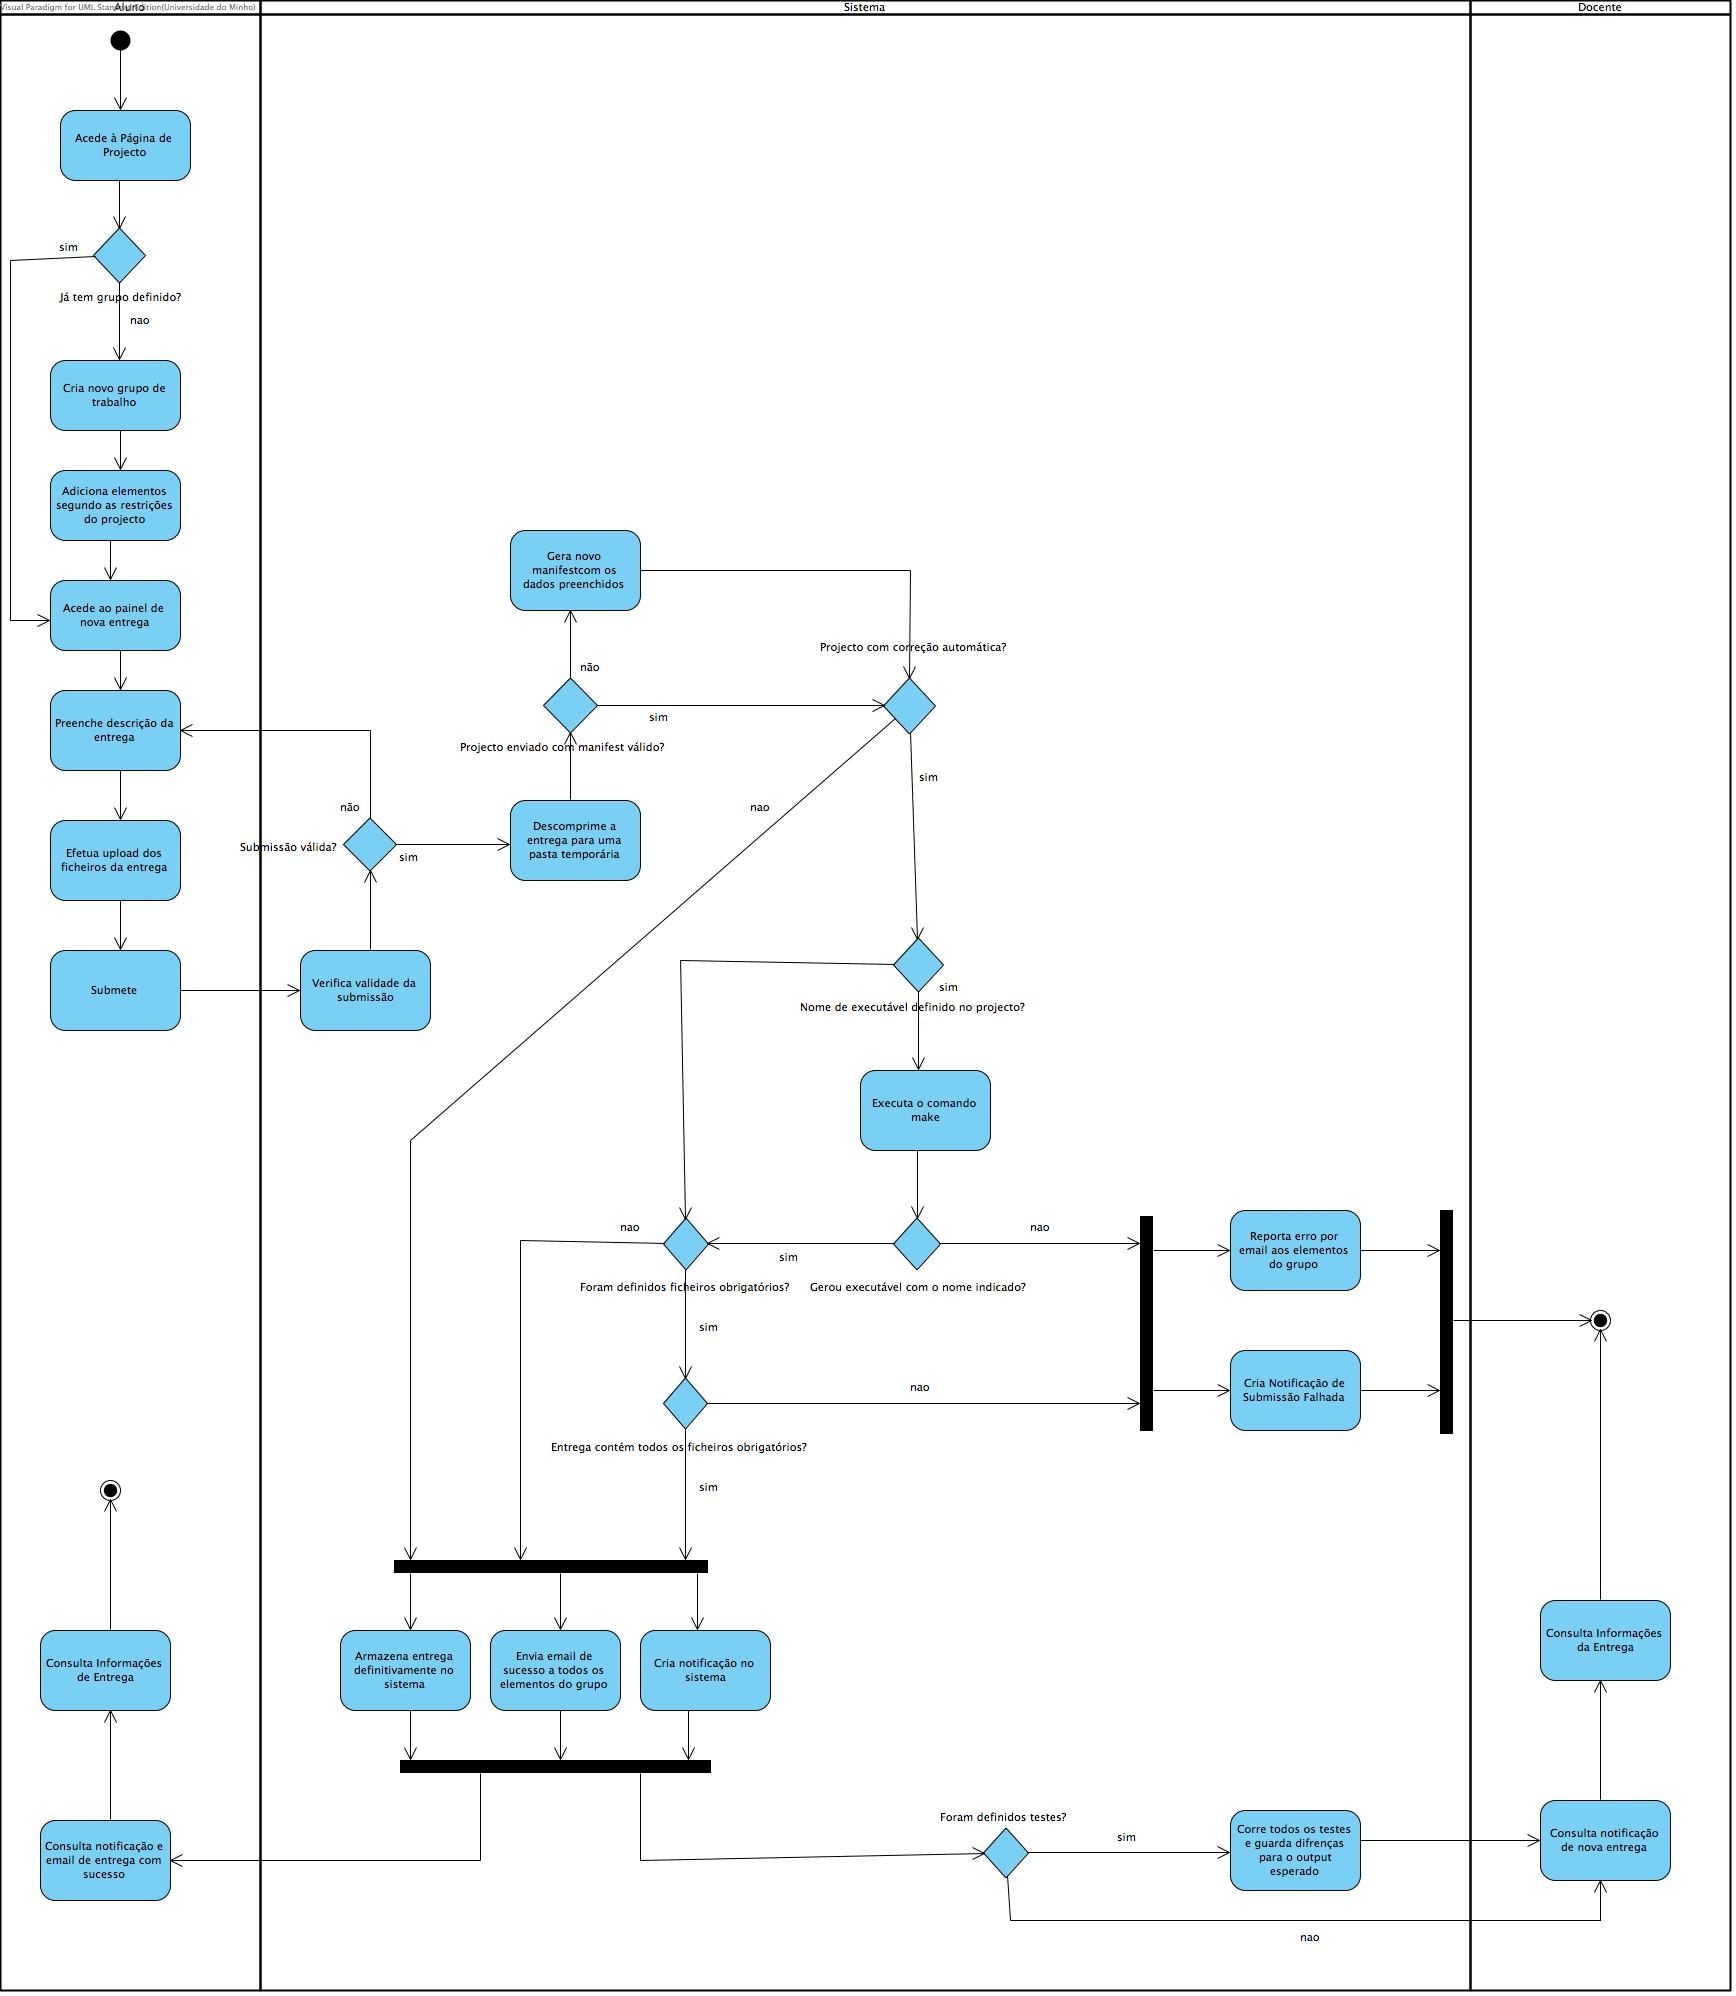
\includegraphics[width=1\textwidth,center]{images/arquitetura/submissao-projecto}
  \caption{Fluxo: Submeter Projeto}
  \label{fig:submissao-projecto}
\end{figure}
